\documentclass[12pt]{article}
\usepackage[margin=1in]{geometry}

\usepackage{latexsym, amssymb, amsmath, amsfonts, amscd, amsthm}
\usepackage{enumerate, hyperref, multicol, tikz}
\usepackage{graphicx}
\graphicspath{{./pictures/}}

\theoremstyle{definition}
\newtheorem{definition}{Definition}
\newtheorem{example}{Example}
\newtheorem{exercise}{Exercise}
\newtheorem{question}{Question}
\newtheorem*{notation*}{Notation}

\newtheorem{fact}{Fact}
\newtheorem{lemma}{Lemma}
\newtheorem{proposition}{Proposition}
\newtheorem{theorem}{Theorem}
\newtheorem{corollary}{Corollary}

\newcommand{\NN}{\mathbb{N}}
\newcommand{\ZZ}{\mathbb{Z}}
\newcommand{\QQ}{\mathbb{Q}}
\newcommand{\RR}{\mathbb{R}}
\newcommand{\CC}{\mathbb{C}}
\newcommand{\FF}{\mathbb{F}}

\begin{document}
\textbf{Alicia Ledesma Alonso}

\begin{exercise} Edelsbrunner Chapter 2, problem 1 \textit{Classifying 2-manifolds}\newline
	Characterize the two surfaces depicted in Figure 11.15 in terms of genus, boundary, and orientability. \begin{center}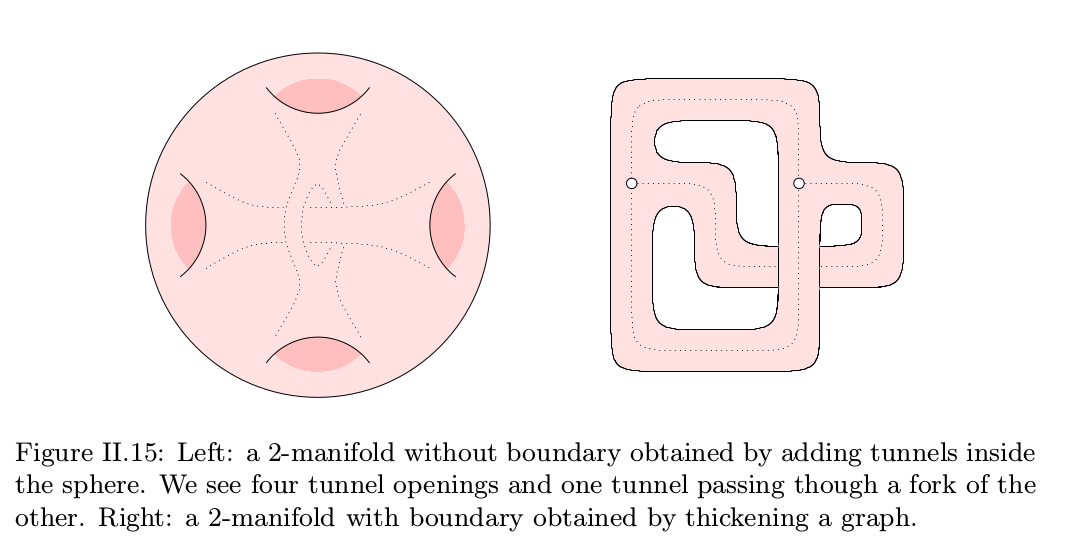
\includegraphics[scale=0.4]{FigureII-15}\end{center} The first manifold to the left has a genus of 3, since three closed curves (cuts) can be made to the manifold before creating two pieces. It has no boundary, but it is orientable. The second manifold to the right has a genus of 2, since two closed curves (cuts) can be made to the manifold before creating two pieces. Notice that the shape looks similar to a double tori except there are two vertices instead of one. The manifold has boundary, and it is orientable. 
\end{exercise}

\begin{exercise} Edelsbrunner Chapter 2, problem 2 \textit{2-coloring}\newline
	Let $K$ be a triangulation of an orientable 2-manifold without boundary. Construct $L$ by decomposing each edge into two and each triangle into six. To do this, we add a new vertex in the interior of each edge. Similarly, we add a new vertex in the interior of each triangle, connecting it to the six vertices in the boundary of the triangle. The resulting structure is the same as the barycentric subdivision of $K$, which we will define in Chapter III.
	\begin{enumerate}[(i)]
		\item Show that the vertices of $L$ can be 3-colored such that no two neighboring vertices recieve the same color. 
		\item Prove that the triangles of $L$ can be 2-colored such that no two triangles sharing an edge receive the same color. 
	\end{enumerate}
\end{exercise}

\begin{exercise} Edelsbrunner Chapter 2, problem 3 \textit{Klein bottle}\newline 
	Cut and paste the standard polygonal schema for the Klein bottle $(a,a,b,b)$ to obtain the polygonal schema in which opposite edges of a square are identified $(a,b,a^-1,b)$; see Figure 11.3.\begin{center}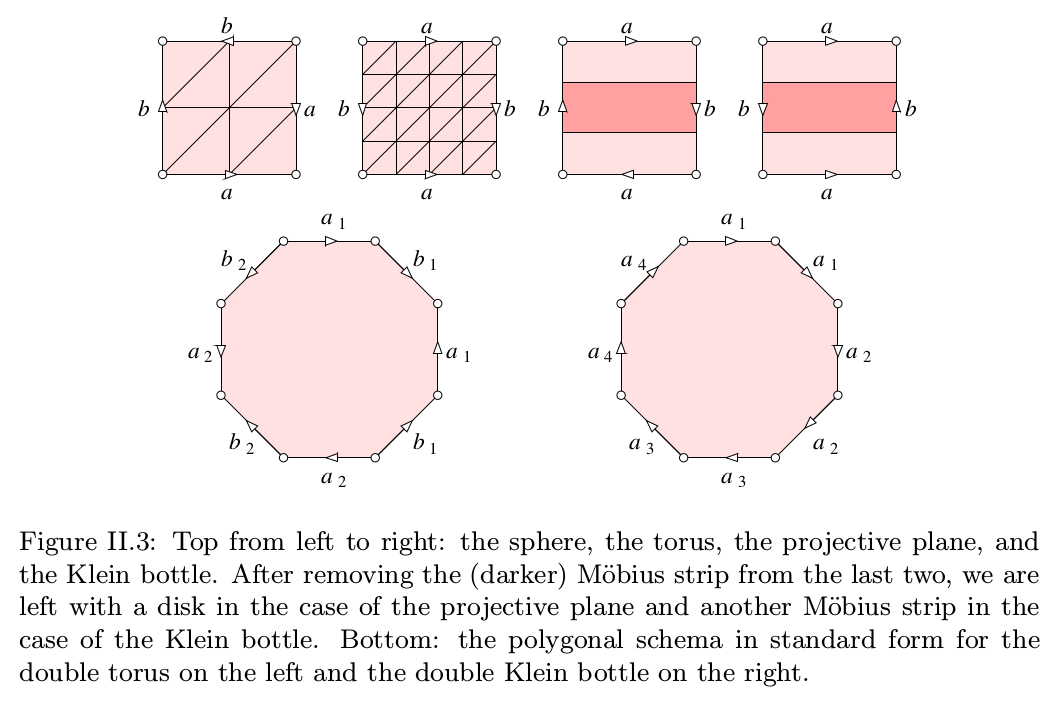
\includegraphics[scale=0.4]{FigureII-3}\end{center}
\end{exercise}

\begin{exercise} Edelsbrunner Chapter 2, problem 4 \textit{Triangulation of 2-manifold}\newline
	Let $V={1,2,...,n}$ be a set of $n$ vertices and $F\subseteq\vec{V,3}$ a set of $l=$ card $F$ triangles. Give an algorithm that takes time at most proportional to $n+l$ for the following tasks:
	\begin{enumerate}[(i)]
		\item decide whether or not every edge is shared by exactly two triangles;
		\item decide wheter or not every vertex belongs to a set of triangles whose union is a disk.
	\end{enumerate}
\end{exercise}

\begin{exercise} Edelsbrunner Chapter 2, problem 5 \textit{Intersection tests in $\mathbb{R}^3$}\newline
	Let $a,b,c\in\mathbb{R}^3$ and $u,v,w\in\mathbb{R}^3$ be the vertices of two triangles in space. Write numerical tests for the following questions:
	\begin{enumerate}[(i)]
		\item does $u$ see $a,b,c$ form a left-turn or a right-turn?
		\item does the line segment with endpoints $u$ and $v$ cross the plan that passes through $a,b,c$?
		\item are the boundaries of the two triangles linked in $\mathbb{R}^3$?
	\end{enumerate}
\end{exercise}

\begin{exercise} Edelsbrunner Chapter 2, problem 6 \textit{Irreducible triangulations}\newline
	An \textit{irreducible} triangulation is one in which every edge contraction changes its topological type. Prove that the only irreducible triangulation of $\mathbb{S}^2$ is the boundary of the tetrahedron, which consists of four triangles sharing six edges and four vertices. 
\end{exercise}

\begin{exercise} Edelsbrunner Chapter 2, problem 7 \textit{Graphs on M\"obius strip}\newline
	Is every graph that can be embedded on the M\"obius strip planar?
\end{exercise}

\begin{exercise} Edelsbrunner Chapter 2, problem 8, \textit{Squared distance minimization}\newline
	Let $S$ be a finite set of points in $\mathbb{R}^3$ and $f:\mathbb{R}^3\to\mathbb{R}$ be defined by $f(x)=\sum_{p\in S} ||x-p||^2$.
	\begin{enumerate}[(i)]
		\item Show that $f$ is a quadratic function and has a unique minimum.
		\item At which point does $f$ attain its minimum?
	\end{enumerate}
\end{exercise}

\end{document}